\chapter{Opis projektnog zadatka}
				
		\section{Uvod}
		Cilj ovog projekta je razviti web aplikaciju koja će značajno ubrzati proces digitalizacije u računovodstvenim tvrtkama. Tradicionalni način obrade dokumenata je gotovo uvijek spor i nepouzdan jer je podložan ljudskim pogreškama. Naša nova aplikacija rješava te probleme te pruža brži, precizniji i pouzdaniji način upravljanja dokumentima. Ključna prednost nad tradicionalnim načinom je povećanje produktivnosti. Korisnici aplikacije će moći obrađivati mnogo veći broj dokumenata u puno kraćem vremenskom periodu, što rezultira značajnim uštedama vremena i resursa uloženih u rad.
		
		\section{Osnovne funkcionalnosti}
		Glavna funkcionalnost ove aplikacije je detekcija dokumenata na slikama čime se eliminira potreba za ručnim označavanjem i kategorizacijom dokumenata. Nakon toga dolazi izvođenje optičkog prepoznavanja teksta (OCR) iz tih dokumenata. Ovaj ključni proces omogućava tvrtki da izvuče vrijedne informacije iz papirnatih dokumenata i prevede ih u digitalni oblik. Sofisticiranim OCR sustavom se može postići vrlo visoka točnost u prepoznavanju teksta. Aplikacija je fleksibilna i skalabilna, omogućit će se korisnicima učitavanje do 50 slika istovremeno.
		
		Značaj ovog projekta je unaprijediti i ubrzati proces digitalizacije dokumenata, osiguravajući točnost i pouzdanost u svakom koraku, od samog skeniranja do arhiviranja. S ovom aplikacijom će se pomoći smanjiti vjerojatnost ljudskih pogrešaka što je od velike važnosti za očuvanje točnosti financijskih podataka, te se time povećava učinkovitost poslovanja.
		
		Prilikom pokretanja aplikacije prikazuje se mogućnost prijave u sustav s postojećim računom za što su potrebni:
		\begin{packed_item}
			\item \text{Korisničko ime}
			\item \text{Zaporka}
		\end{packed_item}

		\textit{slika prijave}
		
		\section{Tehnički aspekti i razvojni ciklus}

		Aplikacija  će biti razvijena korištenjem modernih tehnologija kako bi osigurala visoku razinu sigurnosti i performansi. Backend će biti implementiran pomoću popularnog okvira kao što je Django, osiguravajući robusnost i skalabilnost sustava. Kako bi se postigla brza i responzivna korisnička sučelja, frontend će se temeljiti na Reactu.
		Važan aspekt svake aplikacije je korisničko sučelje koje smo dizajnirali tako da je vrlo intuitivno i jednostavno za korištenje. 
		Dizajnerske odluke temelje se na najboljim praksama kako bi se različitim korisnicima osiguralo ugodno iskustvo.
		Kroz pažljivo planiranje korisničkih tokova i jasnu navigaciju, aplikacija će omogućiti korisnicima brz i učinkovit pristup funkcionalnostima.
		Razvoj će se odvijati u iteracijama koristeći agilne metodologije, što će omogućiti fleksibilnost u prilagodbi promjenama zahtjeva. Redovito testiranje, uključujući testiranje jedinica, integracije i sustava, bit će ključno za osiguravanje stabilnosti i performansi aplikacije.
		
		\section{Prava određenih korisnika}
		
		Prijavom u sustav korisniku se dodjeljuju njegova prava. Svaki korisnik ima osnovne mogućnosti:
		\begin{packed_item}
			\item mijenjanje lozinke korisničkog računa
			\item skeniranje dokumenata
			\item pristup povijesti vlastitih skeniranih dokumenata
			\item Nakon skeniranja dokumenta ima pravo potvrditi njegovu točnost, odnosno odbiti ga.
		\end{packed_item}
		S obzirom na osjetljivost financijskih podataka, sigurnost je ključna komponenta. Pristup određenim funkcionalnostima bit će strogo kontroliran putem sustava ovlasti,
		 osiguravajući da svaki korisnik ima pristup samo onim informacijama i radnjama koje su relevantne za njegovu ulogu.
		\newline
		Dodatna prava koja ovise o njegovu položaju u tvrtki su:
		\begin{packed_item}
			\item \textbf{Zaposlenici:} 
					\begin{packed_item}
						\item Imaju pravo slati svoje skenirane dokumente revizoru.
					\end{packed_item}
			\item \textbf{Revizori:} 
					\begin{packed_item}
						\item Imaju odgovornost za pregled svih pristiglih dokumenata i daljnje usmjeravanje prema računovođama
						\item odbijanje dokumenta ako ne zadovoljava potrebne uvjete 
					\end{packed_item}
			\item \textbf{Računovođe:} 
						\begin{packed_item}
						\item Imaju ključnu ulogu u arhiviranju primljenih dokumenata i dodjeljivanju jedinstvenih brojeva arhivama
						\item slanje dokumenata direktoru na potpis
					\end{packed_item}
			\item \textbf{Direktor:}
						\begin{packed_item} 
							\item Ima najveće ovlasti, potpunu preglednost nad svim dokumentima i statistikama zaposlenika
							\item Pregled povijesti dokumenata i zaposlenika
							\item mogućnost dijeljenja odabranih dokumenata na društvene mreže
							\item Jedini ima mogućnost registriranja novih korisnika, pri čemu on i dodjeljuje ulogu svakom novom korisniku. 
							\item Može i obrisati korisnika koji se nalazi u sustavu iz sustava.
						\end{packed_item}
		\end{packed_item}
		
		\section{Slična rješenja}
		
		Ova aplikacija nije jedina takva na tržištu, slična rješenja uključuju Adobe Acrobat za OCR i upravljanje dokumentima, te ABBYY FineReader za napredno optičko prepoznavanje znakova. No ova aplikacija se razlikuje po svojoj kombinaciji funkcionalnosti. Ona će kombinirati najbolje aspekte ovih rješenja i dodati posebne značajke prilagođene potrebama računovodstva. To uključuje automatsku detekciju i organizaciju dokumenata te više razine pristupa.

		\section{Partnerstva i integracije}

		Staviti ćemo naglasak na uspostavu suradnje s drugim tehnološkim tvrtkama i pružateljima usluga kako bi se proširile funkcionalnosti aplikacije. Partnerstva mogu omogućiti pristup dodatnim resursima, stručnost u specifičnim područjima te ubrzanje inovacija.
		Prvenstveno ćemo se fokusirati na partnere koji se bave područjima naprednog OCR-a, sigurnosnih rješenja ili prilagođenih integracija. Kroz partnerstva i integracije, aplikacija će pružiti dodatnu vrijednost korisnicima. Na primjer, mogućnost sinkronizacije podataka s računovodstvenim softverom ili automatsko prepoznavanje i integraciju informacija iz drugih aplikacija može značajno poboljšati korisničko iskustvo.				 Razvojni tim će redovito pratiti tehničke trendove i inovacije kako bi osigurao da partnerstva i integracije prate najnovije tehnološke standarde. Ova proaktivna pristup osigurat će dugoročnu relevantnost aplikacije u dinamičnom okruženju tehnoloških promjena.
		
		\section{Zaključak}
		
		U konačnici, ovim projektom  stvaraju se temelji za razvoj napredne i inovativne web aplikacije koja će uvelike ubrzati i
		poboljšati proces digitalizacije u računovodstvenim tvrtkama i donijeti korisnicima novo i učinkovito rješenje s
		minimaliziranom količinom pogrešaka za obradu dokumenata. Uz kombinaciju tehnoloških rješenja, sigurnosnih mjera i korisničkih sučelja, očekuje se da će ova aplikacija postati ključni alat u optimizaciji poslovnih operacija. 
		Njezina prilagodljivost i skalabilnost čine je perspektivnim rješenjem koje će unaprijediti digitalizaciju dokumenata na novu razinu.
		Kroz ove aktivnosti, projekt će izgraditi snažnu mrežu podrške i suradnje, čime će osigurati da aplikacija ostane fleksibilna i prilagodljiva promjenama u tehnologiji i zahtjevima korisnika.
		\eject
		
		\section{Primjeri u \LaTeX u}
		
		\text{Ovo potpoglavlje izbrisati.}\\

		U nastavku se nalaze različiti primjeri kako koristiti osnovne funkcionalnosti \LaTeX a koje su potrebne za izradu dokumentacije. Za dodatnu pomoć obratiti se asistentu na projektu ili potražiti upute na sljedećim web sjedištima:
		\begin{itemize}
			\item Upute za izradu diplomskog rada u \LaTeX u - \url{https://www.fer.unizg.hr/_download/repository/LaTeX-upute.pdf}
			\item \LaTeX\ projekt - \url{https://www.latex-project.org/help/}
			\item StackExchange za Tex - \url{https://tex.stackexchange.com/}\\
		
		\end{itemize} 	


		
		\noindent \underbar{podcrtani tekst}, \textbf{podebljani tekst}, 	\textit{nagnuti tekst}\\
		\noindent \normalsize primjer \large primjer \Large primjer \LARGE {primjer} \huge {primjer} \Huge primjer \normalsize
				
		\begin{packed_item}
			
			\item  primjer
			\item  primjer
			\item  primjer
			\item[] \begin{packed_enum}
				\item primjer
				\item[] \begin{packed_enum}
					\item[1.a] primjer
					\item[b] primjer
				\end{packed_enum}
				\item primjer
			\end{packed_enum}
			
		\end{packed_item}
		
		\noindent primjer url-a: \url{https://www.fer.unizg.hr/predmet/proinz/projekt}
		
		\noindent posebni znakovi: \# \$ \% \& \{ \} \_ 
		$|$ $<$ $>$ 
		\^{} 
		\~{} 
		$\backslash$ 
		
		
		\begin{longtblr}[
			label=none,
			entry=none
			]{
				width = \textwidth,
				colspec={|X[8,l]|X[8, l]|X[16, l]|}, 
				rowhead = 1,
			} %definicija širine tablice, širine stupaca, poravnanje i broja redaka naslova tablice
			\hline \SetCell[c=3]{c}{\textbf{naslov unutar tablice}}	 \\ \hline[3pt]
			\SetCell{LightGreen}IDKorisnik & INT	&  	Lorem ipsum dolor sit amet, consectetur adipiscing elit, sed do eiusmod  	\\ \hline
			korisnickoIme	& VARCHAR &   	\\ \hline 
			email & VARCHAR &   \\ \hline 
			ime & VARCHAR	&  		\\ \hline 
			\SetCell{LightBlue} primjer	& VARCHAR &   	\\ \hline 
		\end{longtblr}
		

		\begin{longtblr}[
				caption = {Naslov s referencom izvan tablice},
				entry = {Short Caption},
			]{
				width = \textwidth, 
				colspec = {|X[8,l]|X[8,l]|X[16,l]|}, 
				rowhead = 1,
			}
			\hline
			\SetCell{LightGreen}IDKorisnik & INT	&  	Lorem ipsum dolor sit amet, consectetur adipiscing elit, sed do eiusmod  	\\ \hline
			korisnickoIme	& VARCHAR &   	\\ \hline 
			email & VARCHAR &   \\ \hline 
			ime & VARCHAR	&  		\\ \hline 
			\SetCell{LightBlue} primjer	& VARCHAR &   	\\ \hline 
		\end{longtblr}
	


		
		
		%unos slike
		\begin{figure}[H]
			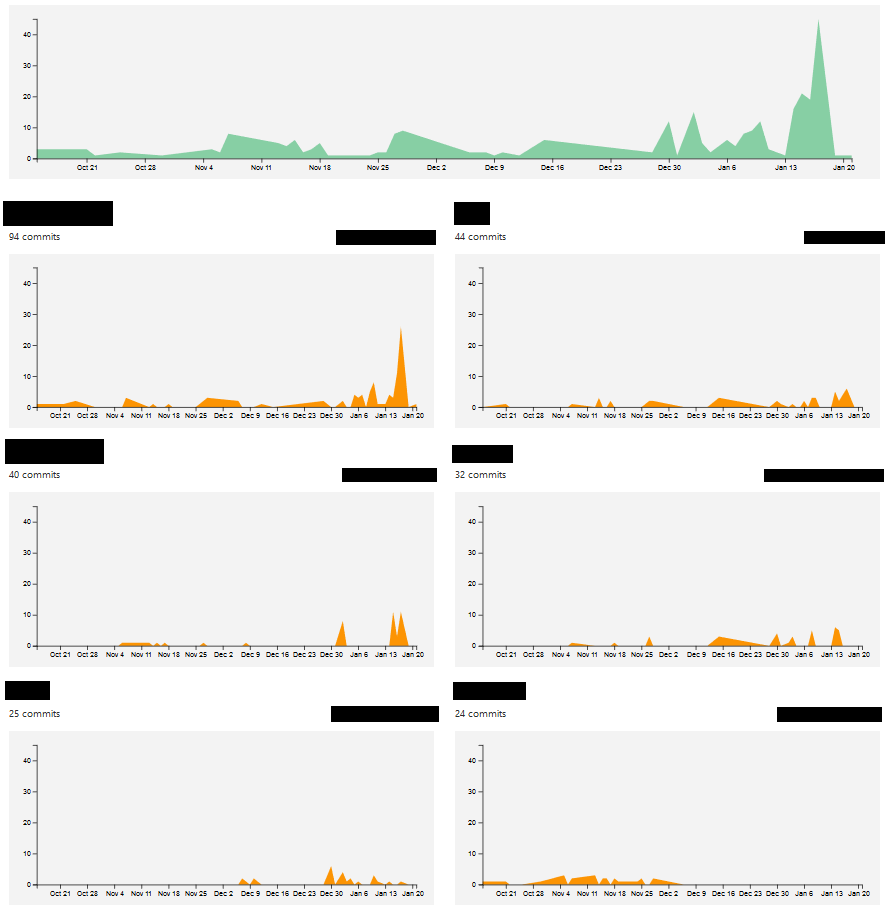
\includegraphics[scale=0.4]{slike/aktivnost.PNG} %veličina slike u odnosu na originalnu datoteku i pozicija slike
			\centering
			\caption{Primjer slike s potpisom}
			\label{fig:promjene}
		\end{figure}
		
		\begin{figure}[H]
			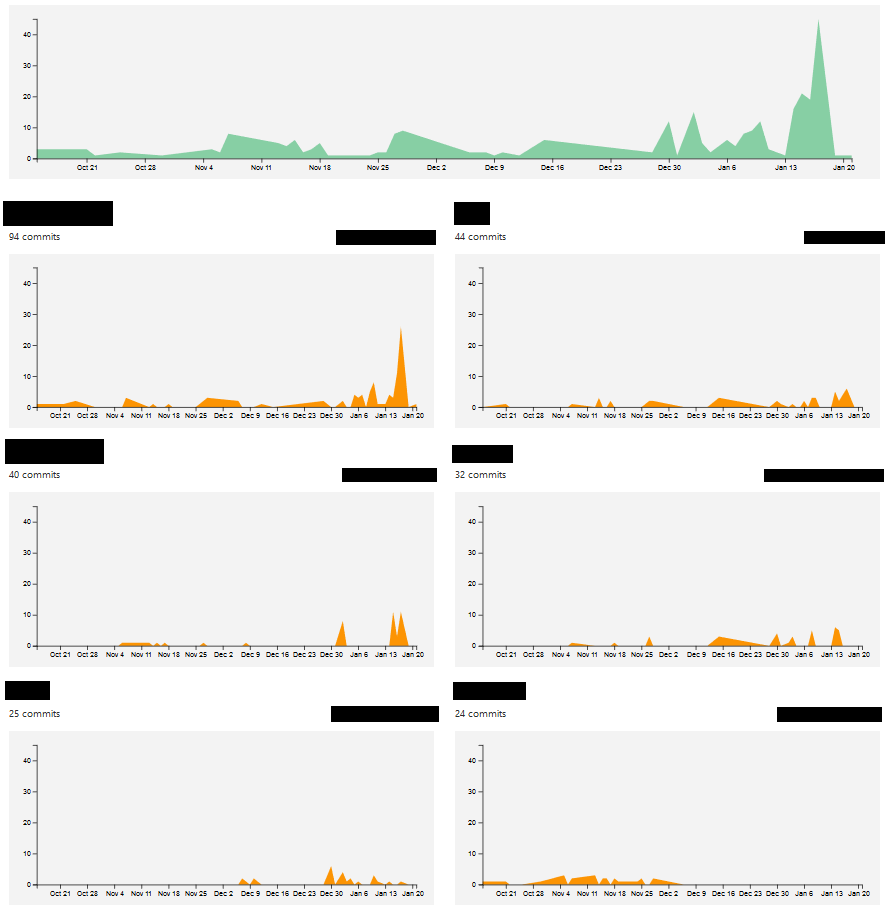
\includegraphics[width=\textwidth]{slike/aktivnost.PNG} %veličina u odnosu na širinu linije
			\caption{Primjer slike s potpisom 2}
			\label{fig:promjene2} %label mora biti drugaciji za svaku sliku
		\end{figure}
		
		Referenciranje slike \ref{fig:promjene2} u tekstu.
		
		\eject
		
	